\documentclass[10pt]{beamer}

%%%
% STANDARD PREAMBLE
%%%
%https://tex.stackexchange.com/questions/68821/is-it-possible-to-create-a-latex-preamble-header
\usepackage{./beamer_preamble_for_MSU_talk}

\usepackage{subcaption}


%%%
% AGENDA STANDOUT SLIDES
%%%
% Each section-divider standout slide shows the whole outline, with the current
% topic highlighted.  The outline lives in ONE place -- \agendatopics below.
% To show it, call \agendaframe{<n>}, where <n> is the topic's position in the list.

\newcounter{agendaindex}
\newcounter{agendacurrent}

% THE OUTLINE.  One \agendaentry per topic, in presentation order.
\newcommand{\agendatopics}{%
	\agendaentry{Course Overview}%
	\agendaentry{Why Active Learning?}%
	\agendaentry{About Me}%
	\agendaentry{Discrete Math In Practice: Examples From Machine Learning}%
	\agendaentry{Virtues Of Discrete Math}%
	\agendaentry{How To Read Math}%
}

\newcommand{\agendaentry}[1]{%
	\stepcounter{agendaindex}%
	\ifnum\value{agendaindex}=\value{agendacurrent}%
		\alert{#1}%
	\else
		\textcolor{fg!40!bg}{#1}%
	\fi
	\par\vspace{0.5em}%
}

\newcommand{\agendaframe}[1]{%
	\setcounter{agendacurrent}{#1}%
	\setcounter{agendaindex}{0}%
	\begin{frame}[standout]
		\begin{minipage}{0.92\textwidth}
			\centering
			\agendatopics
		\end{minipage}
	\end{frame}%
}



\begin{document}




\title{CSCI 246 -- Discrete Structures} 
\author{Mike Wojnowicz}

\institute{Montana State University}

\date{Fall 2026}{}



%\begin{frame}[plain, noframenumbering]
%\begin{multicols}{2}
%  \tableofcontents
%\end{multicols}
%\end{frame}

\renewcommand{\insertframenumber}{}


\begin{frame}[plain,label=title-page, noframenumbering ]
  \titlepage
\end{frame}


%
%\begin{frame}{CSCI 246 -- Discrete Structures}
%
% \begin{block}{Delayed start}
% 
%We will start at 4:15 today due to the last-minute room change.
%
%\vspace{0.2cm}
%
%Feel free to 
%\begin{itemize}
%\item Check out the syllabus ahead of time on Canvas
%\item Meet a neighbor
%\item Meditate
%\item Brag to your friends about how much you're going to learn about discrete structures!	
%\item [...]
%\end{itemize}
%
%\end{block}
%	
%\end{frame}




\agendaframe{1}




\begin{frame}{What is Discrete Math?}
\begin{center}
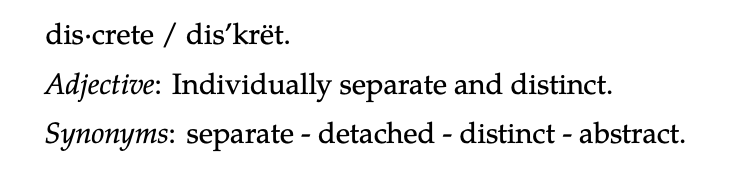
\includegraphics[width=0.9\textwidth]{images/what_is_discrete_math} \\
\end{center}
\pause 
\vspace{1cm}
\begin{center}
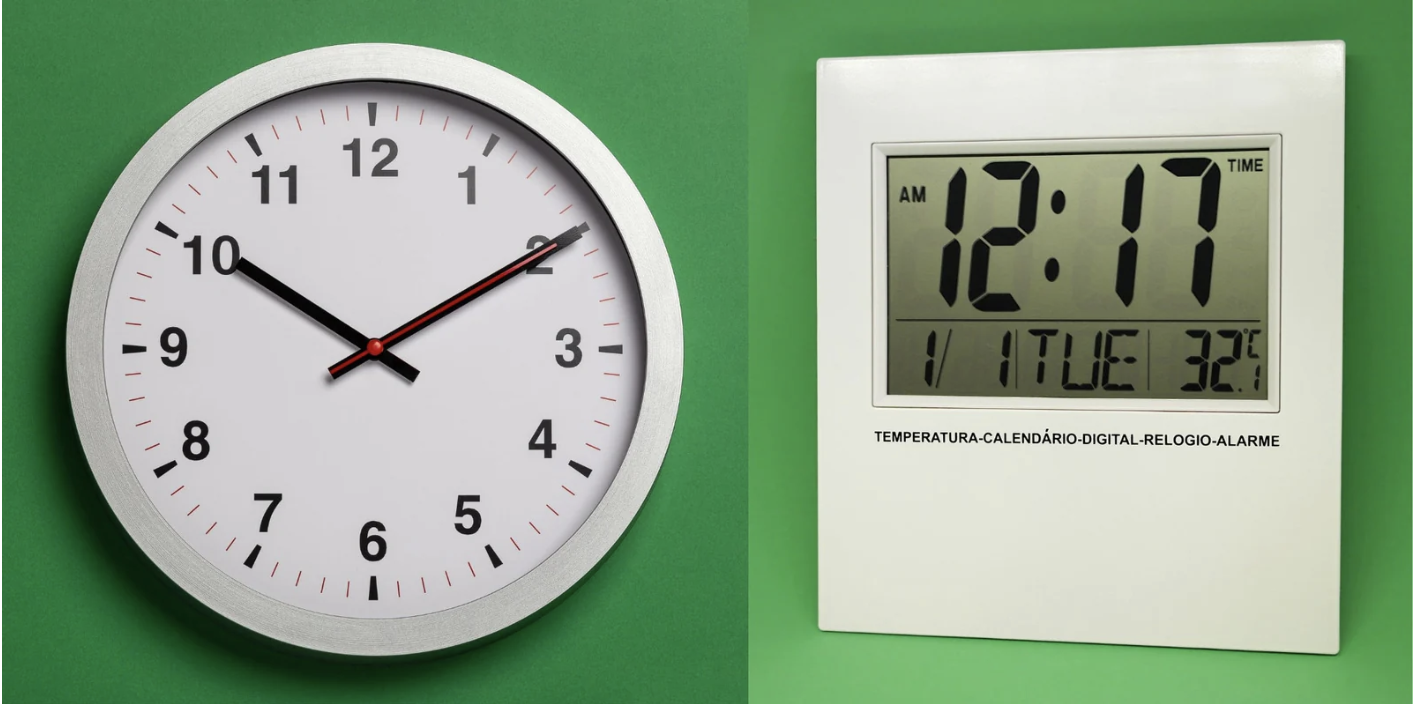
\includegraphics[width=0.6\textwidth]{images/clocks}
\end{center}
\end{frame}


\begin{frame}{Syllabus Review}

\Large \centering
See \color{blue} \underline{\href{https://montana.instructure.com/courses/20155/pages/home-page}{Canvas}} \color{black} for syllabus.

\end{frame}


\agendaframe{2}
 
\begin{frame}{Why Active Learning?}


\begin{figure}[h!]
    \centering

    \begin{subfigure}{0.5\textwidth}
        \centering
        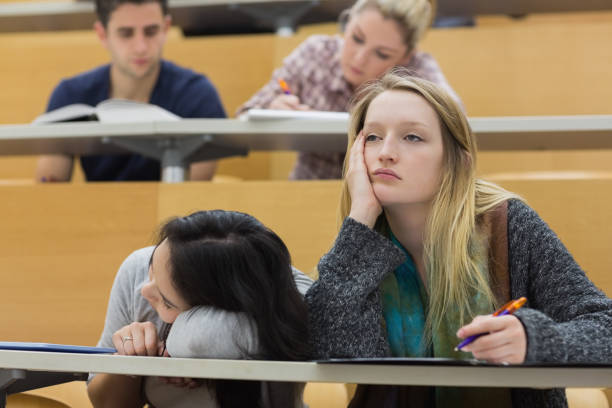
\includegraphics[width=.9\textwidth]{images/bored_student} 
    \end{subfigure}

    \vspace{1cm}
    
    \begin{subfigure}{0.45\textwidth}
        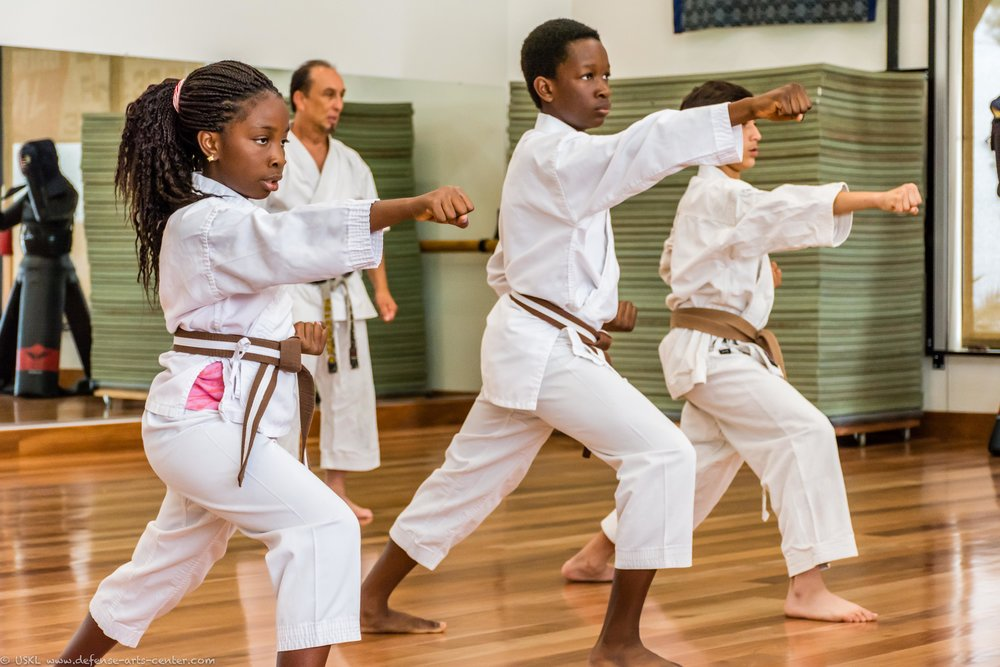
\includegraphics[width=0.9\textwidth]{images/karate} 
 
    \end{subfigure}
    \hfill
    \begin{subfigure}{0.45\textwidth}
        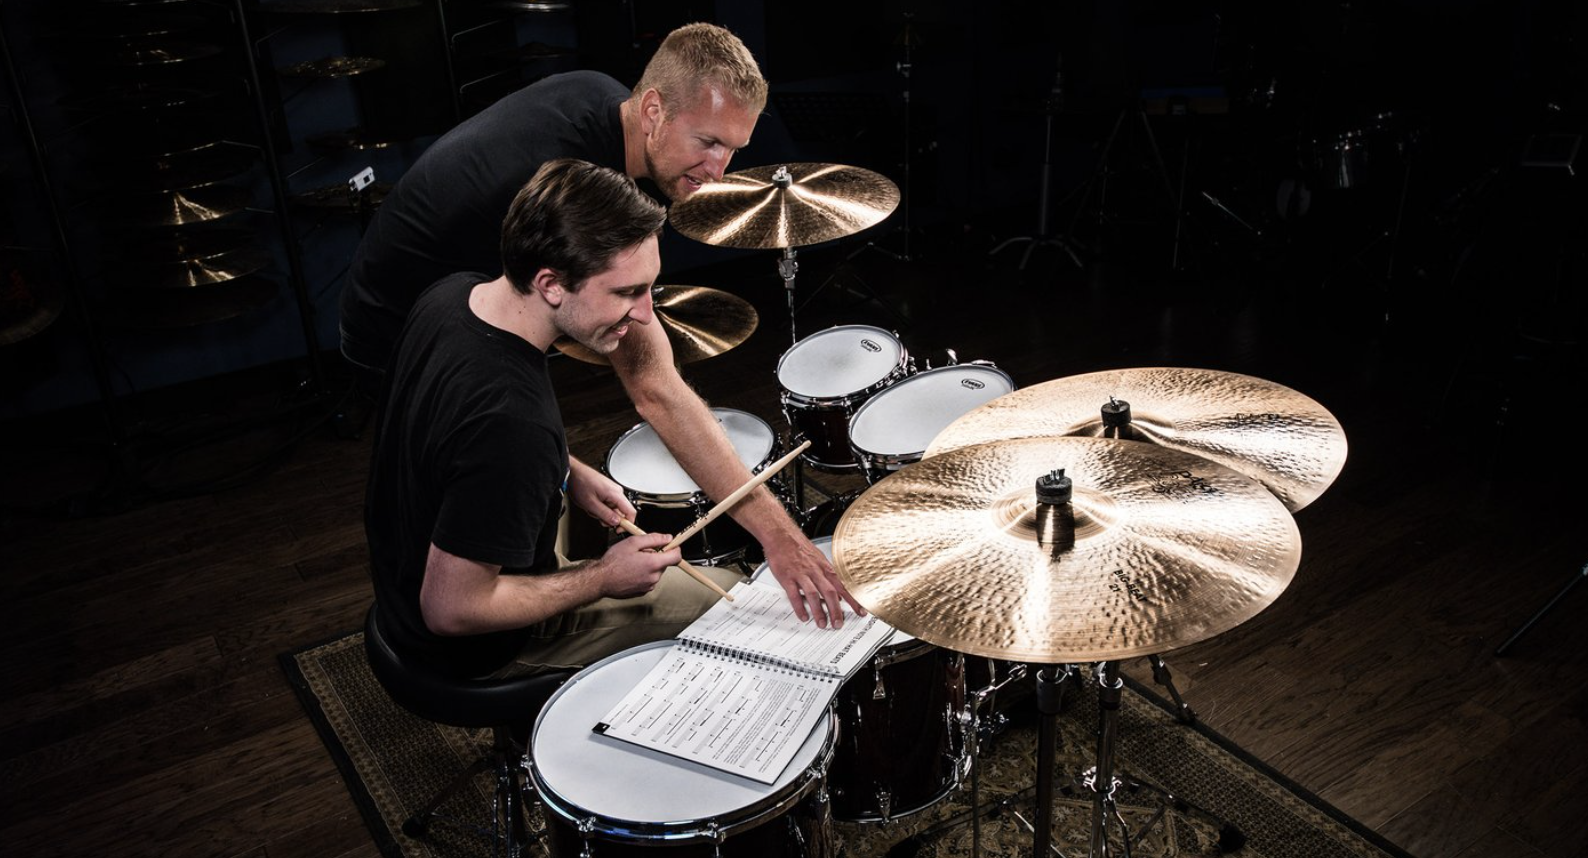
\includegraphics[width=0.9\textwidth]{images/drums} 

    \end{subfigure}
    
\end{figure}
	
\end{frame}




\begin{frame}{Why Active Learning?}
    \begin{figure}
        \centering
        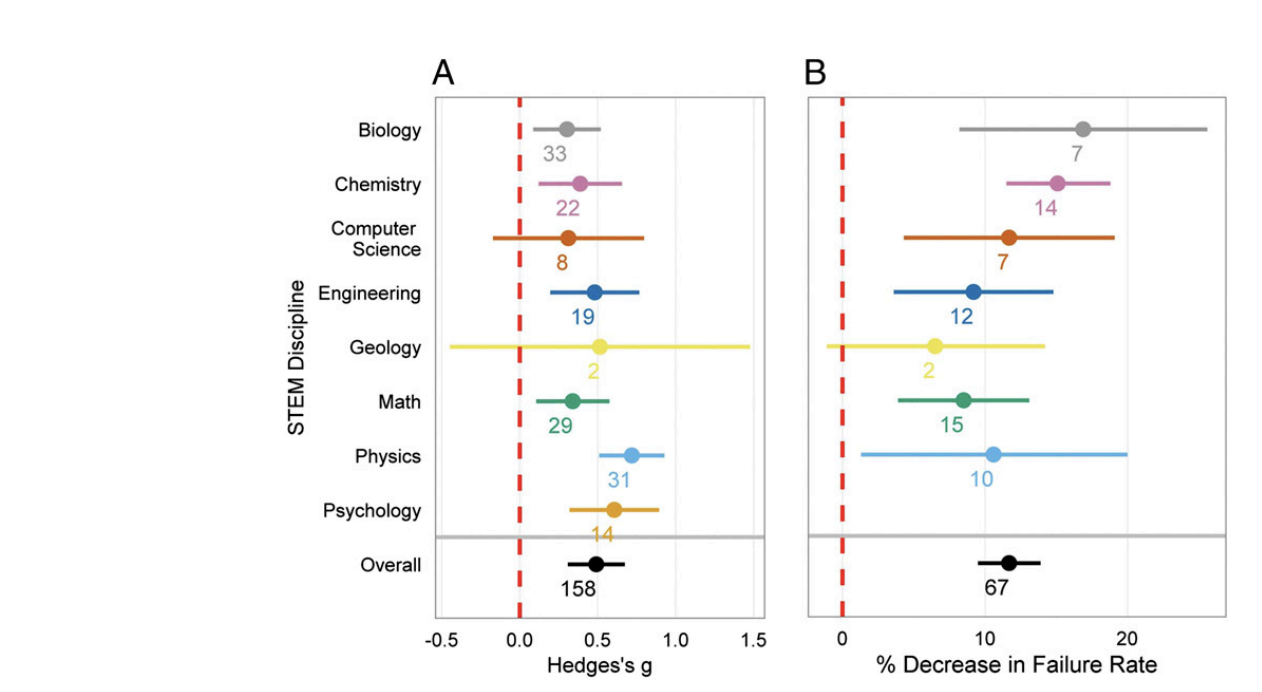
\includegraphics[width=\textwidth]{images/active_learning} 
    \end{figure}
	\citebottom{\hfill Freeman et al. (2014). \textit{Proceedings of the National Academy of Sciences}. \hfill }
\end{frame}






\agendaframe{3}
 
 
\begin{frame}{About Me}
    \begin{columns}[T,onlytextwidth]
        \begin{column}{0.58\textwidth}
            \centering
        	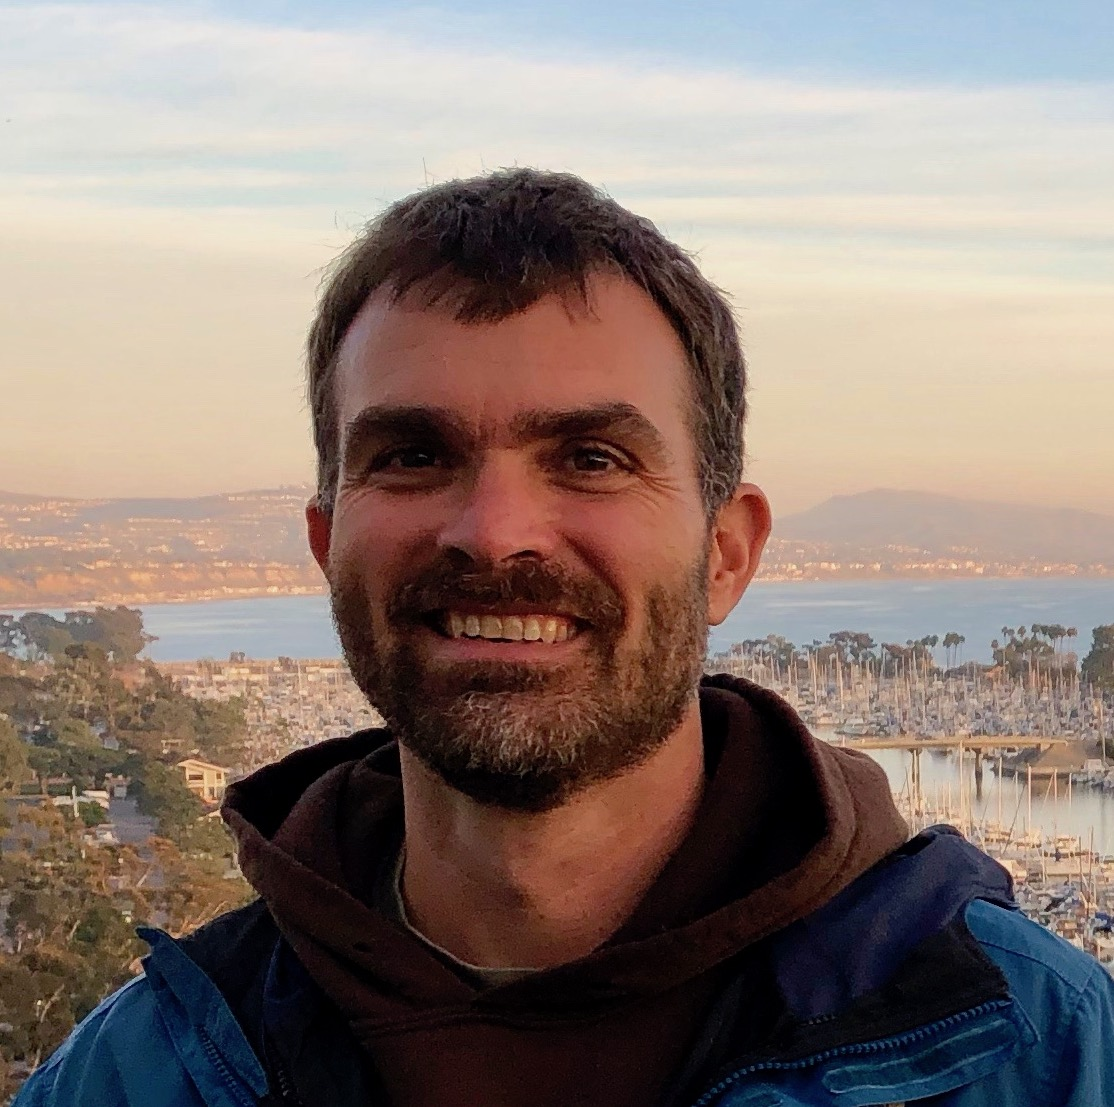
\includegraphics[width=4cm]{images/profile.jpeg}
            \vfill
            Michael Wojnowicz \\
            Assistant Professor, GSoC @ MSU \\
            Research Associate, Biostats @ Harvard \\
            Postdoc, Machine Learning (CS) @ Tufts  \\
			Distinguished Data Scientist @ Cylance \\
			(cybersecurity start-up, sold for \$1.4b) 
			PhD @ Cornell \\
        \end{column}
        \only<2->{
        \begin{column}{0.38\textwidth}
            \centering
            \vspace{0.5in}\textbf{Research interests}
            \begin{itemize}
            \item Probabilistic machine learning
            \item Scalable inference
            \item Modeling spatiotemporal data	
            \end{itemize}
        \end{column}
        }
    \end{columns}
\end{frame}


\begin{frame}

    \begin{figure}
        \centering
        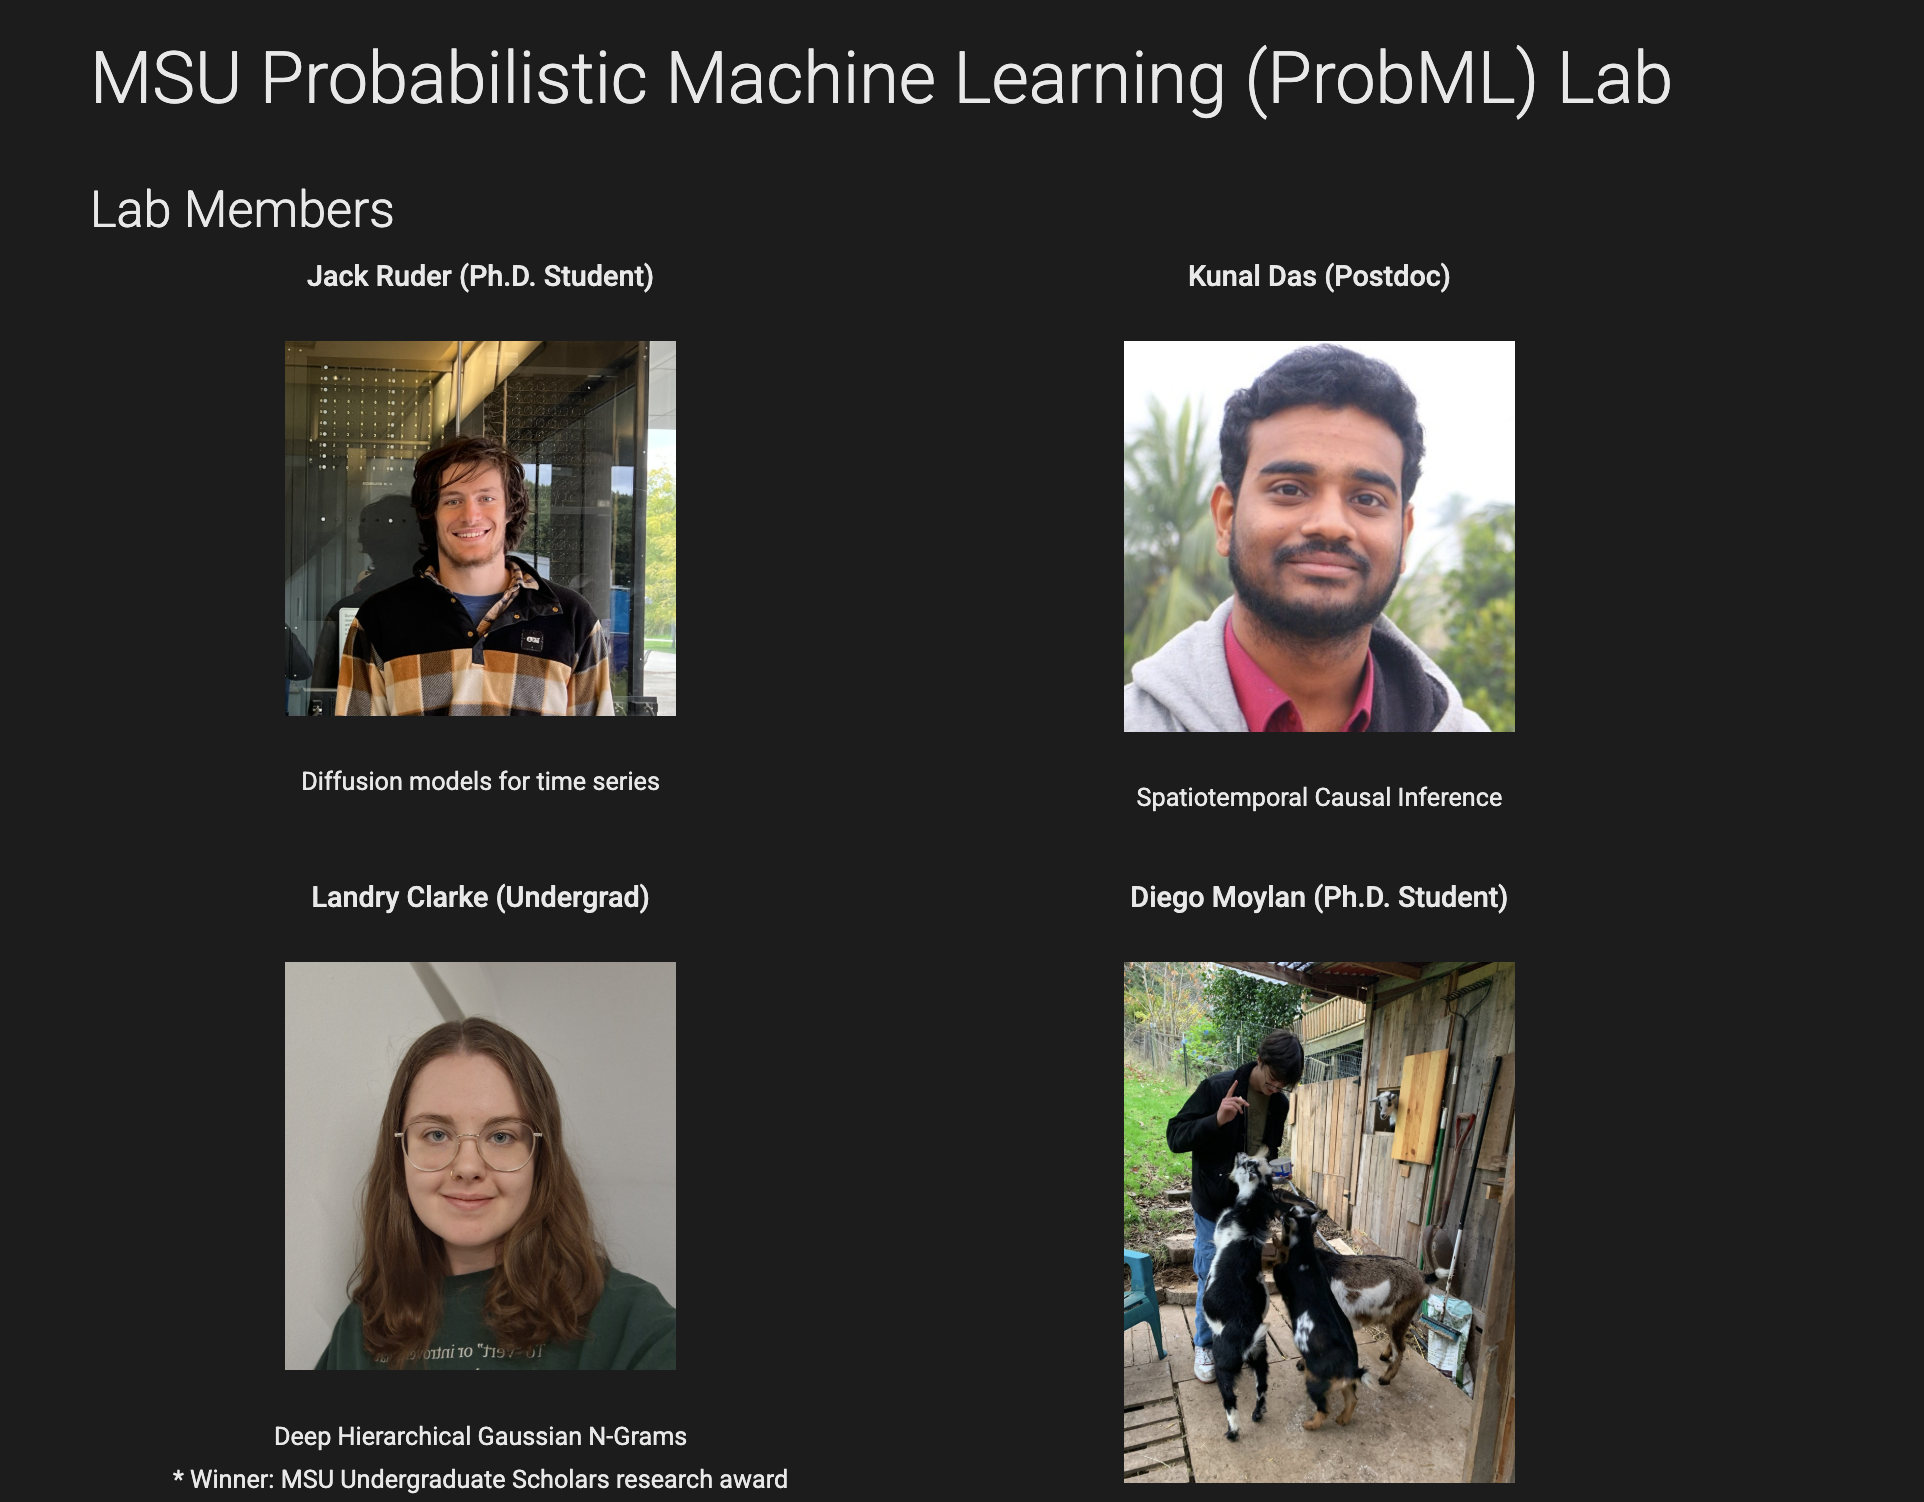
\includegraphics[width=\textwidth]{images/probml_lab} 
    \end{figure}
\pause 
My role: 30\% teaching, 60\% research, 10\% service. 
\end{frame}


\agendaframe{4}


%\begin{frame}{Motivation}
%
%\begin{columns}[c,onlytextwidth]
%    \begin{column}{0.48\textwidth}
%        \centering
%		\begin{figure}
%	   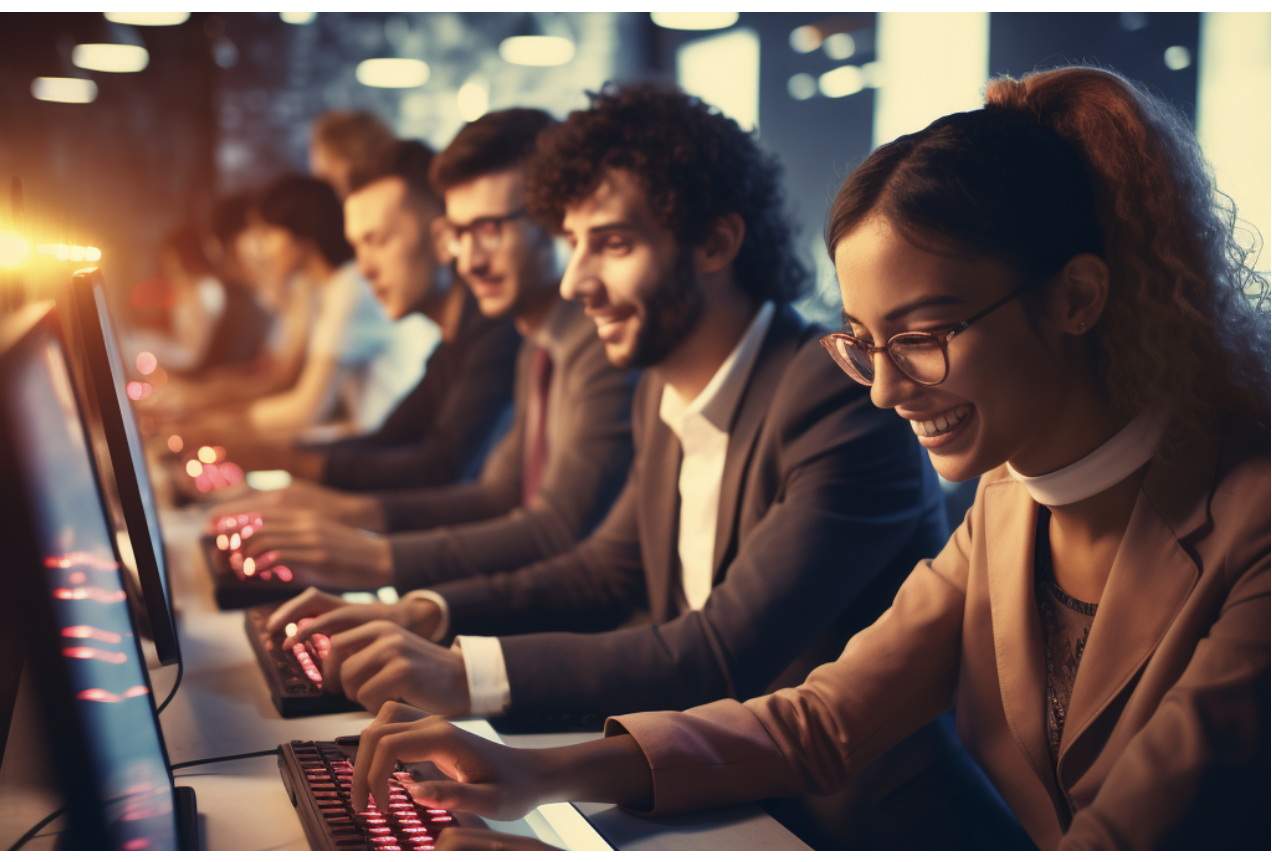
\includegraphics[width=0.9\textwidth]{images/cont_auth}
%	   \vfill 
%	   \textbf{Continuous authentication}:  continuously verify a user’s identity as being authentically theirs throughout their entire interaction with a digital system. 
%		\end{figure}
%    \end{column}
%    \pause 
%    \begin{column}{0.48\textwidth}
%        \centering
%		\vfill 
%	  \begin{tabular}{cc}
%	 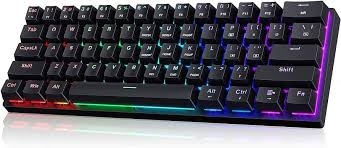
\includegraphics[width=0.5\textwidth]{images/keyboard} & 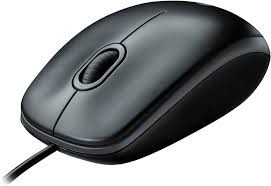
\includegraphics[width=0.5\textwidth]{images/mouse} 
%	  \\
% 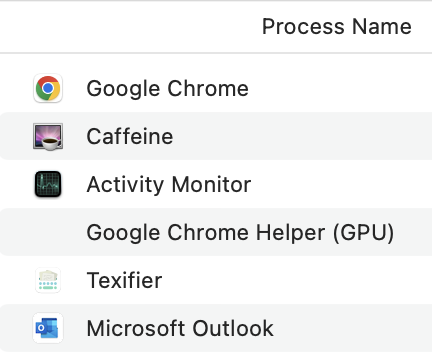
\includegraphics[width=0.5\textwidth]{images/activity_monitor} &
%  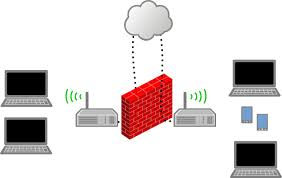
\includegraphics[width=0.5\textwidth]{images/network_traffic} 	
%	  \end{tabular}
%		\textbf{Data sources}: Keystrokes, \\
%		mouse movements, \\ process starts, network traffic, etc.
%    \end{column}
% \end{columns} 
% \pause 
% \vfill 
% \vfill 
% \textbf{Modeling Desiderata}: fast, lightweight, reliable training; interpretable probabilistic (but expressive) models 
%\end{frame}
%



\begin{frame}{Problem \#1: Continuous Authentication}

\begin{columns}[T,onlytextwidth]
    \begin{column}{0.48\textwidth}
        \centering
		\begin{figure}
	   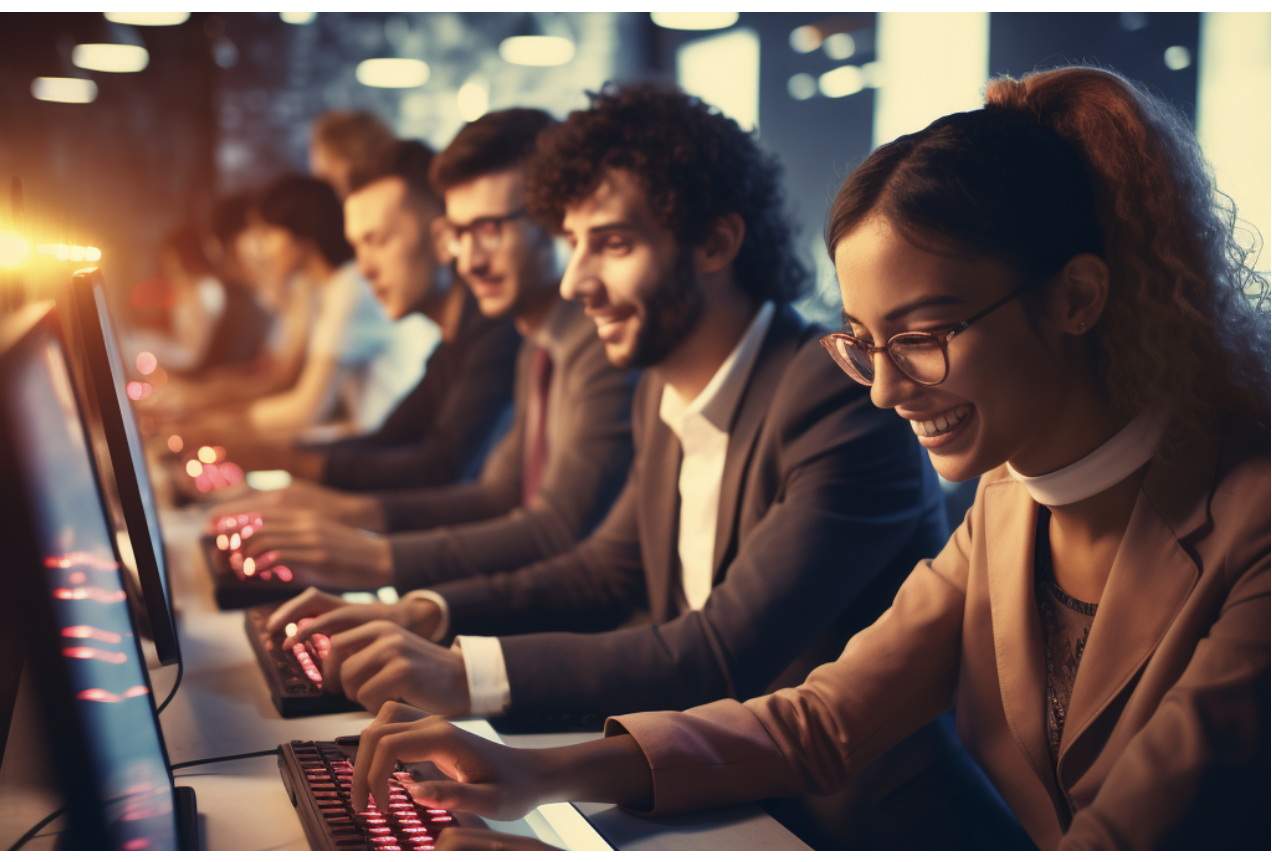
\includegraphics[width=0.9\textwidth]{images/cont_auth}
	   \vfill 
	   \textbf{Continuous authentication}:  continuously verify a user’s identity as being authentically theirs throughout their entire interaction with a digital system. 
		\end{figure}
    \end{column}
    \only<2->{
    \begin{column}{0.48\textwidth}
        \centering

	  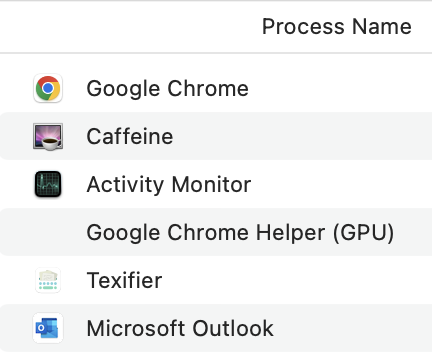
\includegraphics[width=0.9\textwidth]{images/activity_monitor} \\
	  \vfill 
		\textbf{Subgoal}: Learn computer process start sequences which characterize the typical behavior of a user.
    \end{column}
    }
 \end{columns} 
 
  \pause
 \vfill 
  \textbf{Difficulty:} Many 1000s of computer processes, sparsely observed. 
  
 \pause
 \vfill 
  \textbf{Modeling Desiderata}: probabilistic model with fast, reliable training

\end{frame}


%\begin{frame}{Solution: Scalable Bayesian Categorical Modeling}
%\pause 
%\begin{figure}
%\centering
%\caption{A new model for a computer user's process starts (with 1,553 categories, 1,553 covariates, and 17,724 examples), to aid in   \textbf{intruder detection}.} 
%\pause 
%\begin{tabular}{ cl}
%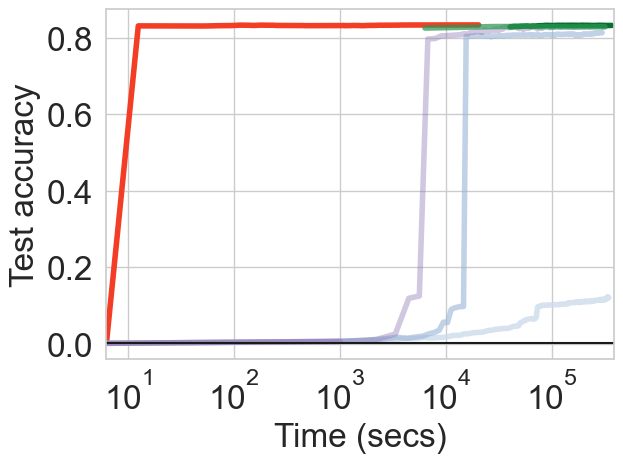
\includegraphics[height=2.3cm]{images/perf_over_time/test_accuracy_cyber_346_show_CB_logit=True_legend=False.png}  
%& 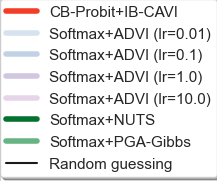
\includegraphics[height=2.3cm]{images/perf_over_time/legend_only_show_CB_logit=False.png} \\
%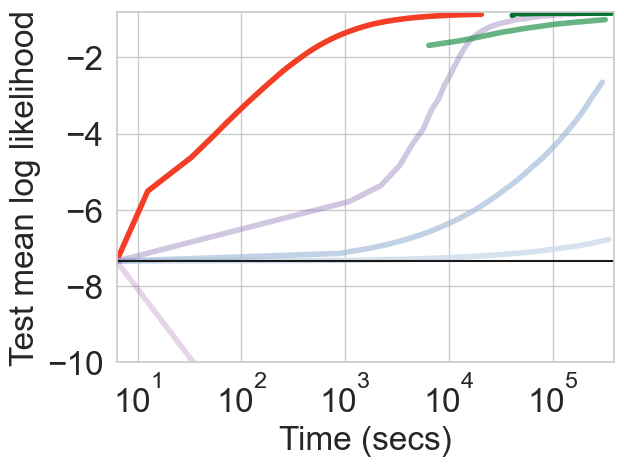
\includegraphics[height=2.8cm]{images/perf_over_time/test_mean_log_likelihood_cyber_346_show_CB_logit=True_legend=False.png} & 
%\end{tabular}
%\label{fig:evaluation}
%\end{figure}
%{\tikz[remember picture,overlay]{
%        \node [draw, rectangle callout, fill=blue!10, align=left, callout relative pointer={(1,0)}, callout pointer shorten=.7cm]  at (0.4, 5.3) {\footnotesize Indistinguishable \\ \footnotesize accuracy.};}}%
%{\tikz[remember picture,overlay]{
%        \node [draw, rectangle callout, fill=blue!10, align=left, callout relative pointer={(1,0)}, callout pointer shorten=.7cm]  at (0.4, 2.3) {\footnotesize Little-to-no \\ \footnotesize cost in \\ \footnotesize probabilities.};}}%       
%{\tikz[remember picture,overlay]{
%        \node [draw,  rectangle callout, fill=red!10, align=left, callout relative pointer={(0,-1)}, callout pointer shorten=.9cm]  at (3.95,1.5) {\tiny 15 mins};}}%
%{\tikz[remember picture,overlay]{
%        \node [draw,  rectangle callout, fill=red!10, align=left, callout relative pointer={(0,-1)}, callout pointer shorten=.9cm]  at (5.2,1.5) {\tiny 24 hrs.};}}%
%{\tikz[remember picture,overlay]{
%        \node [draw,  rectangle callout, fill=red!10, align=left, callout relative pointer={(-1,0)}, callout pointer shorten=.7cm]  at (9.75,5.7) {\scriptsize A new model}}}%
%%
%%\pause 
%%{\tikz[remember picture,overlay]{
%%        \node [draw,  rounded rectangle, fill=green!10, align=left]  at (8.20, 1.8) {\footnotesize These are the results even \\ \footnotesize \textit{before} exploiting parallelism.};}}%
%%\footnotesize 
%%\red{Our method} delivers \textbf{similar predictive performance} in \textbf{far less time}. \\
%%Bio Application: Scalably modeling genetic mutation channels
%\bottomtext{\hfill Wojnowicz, Miller, Aeron, Hughes, `22, \textit{International Conference of Machine Learning (ICML)}.}
%\end{frame}
%


\begin{frame}[label=we-use-course-topics,standout]

\large \centering
The solution to this problem used almost every content area we're covering in this course

\vfill 
\begin{itemize}
	\item Discrete probability and counting
	\item Complexity (Big-O notation)
	\item Recursions
	\item Graph theory
	\item Proof techniques
\end{itemize}
\vfill 
\pause 
\alert{Can you explain why?}
\end{frame}


\begin{frame}{Problem \#2: Early Cancer Detection}

\begin{columns}[T,onlytextwidth]
    \begin{column}{0.46\textwidth}
        \centering
        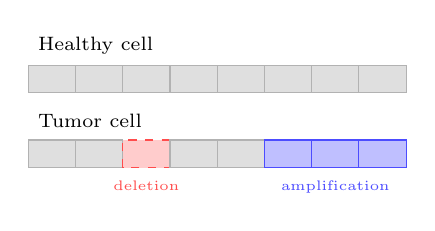
\begin{tikzpicture}
          % --- healthy genome: uniform copy number ---
          \node[anchor=west,font=\scriptsize] at (0,1.45) {Healthy cell};
          \foreach \i in {0,...,7} \draw[fill=gray!25,draw=gray!60] (0.6*\i,0.85) rectangle (0.6*\i+0.6,1.2);
          % --- tumor genome: segments gained and lost ---
          \node[anchor=west,font=\scriptsize] at (0,0.5) {Tumor cell};
          \foreach \i in {0,1} \draw[fill=gray!25,draw=gray!60] (0.6*\i,-0.1) rectangle (0.6*\i+0.6,0.25);
          \draw[fill=red!20,draw=red!70,dashed]              (1.2,-0.1) rectangle (1.8,0.25);
          \foreach \i in {3,4} \draw[fill=gray!25,draw=gray!60] (0.6*\i,-0.1) rectangle (0.6*\i+0.6,0.25);
          \foreach \i in {5,6,7} \draw[fill=blue!25,draw=blue!70] (0.6*\i,-0.1) rectangle (0.6*\i+0.6,0.25);
          \node[red!70,font=\tiny,anchor=north]  at (1.5,-0.15) {deletion};
          \node[blue!70,font=\tiny,anchor=north] at (3.9,-0.15) {amplification};
        \end{tikzpicture}

        \vfill
        \textbf{Somatic copy number alterations (SCNAs)}: tumors gain and lose whole \emph{segments} of DNA, carving the genome into contiguous blocks, each at its own copy number.
    \end{column}
    \only<2->{
    \begin{column}{0.50\textwidth}
        \centering
        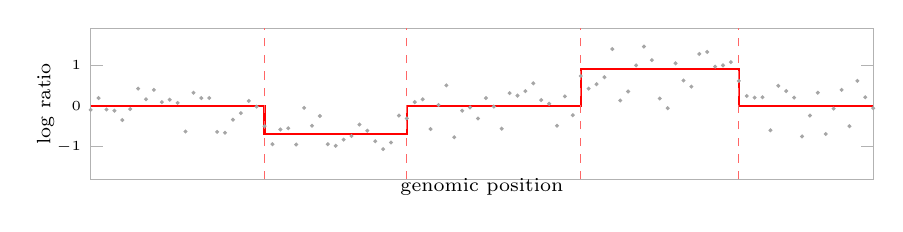
\begin{tikzpicture}
        \begin{axis}[
            width=0.95\linewidth, height=3.5cm,
            xlabel={\scriptsize genomic position}, ylabel={\scriptsize log ratio},
            xmin=0, xmax=99, ymin=-1.8, ymax=1.9,
            xtick=\empty, ytick={-1,0,1},
            tick label style={font=\tiny}, label style={font=\tiny},
            ylabel style={yshift=-6pt}, xlabel style={yshift=4pt},
            axis line style={gray!60}, tick style={gray!60},
        ]
        \addplot[only marks, mark=*, mark size=0.5pt, gray!70] coordinates {
        (0,-0.10) (1,0.19) (2,-0.09) (3,-0.12) (4,-0.35) (5,-0.08) (6,0.42) (7,0.16) (8,0.39)
        (9,0.09) (10,0.15) (11,0.07) (12,-0.63) (13,0.32) (14,0.19) (15,0.19) (16,-0.64)
        (17,-0.66) (18,-0.34) (19,-0.18) (20,0.12) (21,-0.02) (22,-0.50) (23,-0.94) (24,-0.58)
        (25,-0.55) (26,-0.95) (27,-0.05) (28,-0.49) (29,-0.25) (30,-0.94) (31,-0.98) (32,-0.83)
        (33,-0.74) (34,-0.46) (35,-0.61) (36,-0.87) (37,-1.06) (38,-0.90) (39,-0.24) (40,-0.31)
        (41,0.09) (42,0.16) (43,-0.57) (44,0.02) (45,0.50) (46,-0.77) (47,-0.12) (48,-0.04)
        (49,-0.31) (50,0.19) (51,-0.02) (52,-0.56) (53,0.31) (54,0.25) (55,0.36) (56,0.55)
        (57,0.14) (58,0.05) (59,-0.49) (60,0.23) (61,-0.23) (62,0.73) (63,0.42) (64,0.53)
        (65,0.70) (66,1.39) (67,0.13) (68,0.35) (69,0.99) (70,1.45) (71,1.12) (72,0.18) (73,-0.06)
        (74,1.04) (75,0.62) (76,0.47) (77,1.27) (78,1.32) (79,0.96) (80,0.99) (81,1.07) (82,0.61)
        (83,0.24) (84,0.20) (85,0.21) (86,-0.60) (87,0.49) (88,0.36) (89,0.20) (90,-0.75)
        (91,-0.24) (92,0.32) (93,-0.69) (94,-0.07) (95,0.39) (96,-0.50) (97,0.61) (98,0.21)
        (99,-0.06)
        };
        \only<3->{
        \addplot[red, thick, const plot] coordinates {(0,0) (22,-0.7) (40,0) (62,0.9) (82,0) (99,0)};
        \draw[red!60,dashed,thin] (axis cs:22,-1.8) -- (axis cs:22,1.9);
        \draw[red!60,dashed,thin] (axis cs:40,-1.8) -- (axis cs:40,1.9);
        \draw[red!60,dashed,thin] (axis cs:62,-1.8) -- (axis cs:62,1.9);
        \draw[red!60,dashed,thin] (axis cs:82,-1.8) -- (axis cs:82,1.9);
        }
        \end{axis}
        \end{tikzpicture}

        \vfill
        \textbf{Subgoal}: From a noisy sequencing signal, recover the \emph{changepoints} --- the boundaries where copy number jumps.
    \end{column}
    }
 \end{columns}

 \pause
 \pause
 \vfill
  \textbf{Difficulty:} Millions of genomic positions, a faint signal buried in noise, and exponentially many ways to segment them.

 \pause
 \vfill
  \textbf{Modeling Desiderata}: probabilistic model that is accurate at low signal-to-noise, yet fast enough to scale

\end{frame}

\againframe[standout]{we-use-course-topics}


\agendaframe{5}

\begin{frame}{Virtues of developing mathematical reasoning (generally)}

\begin{itemize}
\item Enhances performance studying \textit{any} domain -- not only computer science, but also cybersecurity, sociology, etc.  \pause 
\item Enhances performance at work -- often, math gets the job done better. \pause 
\item \$\$\$ \pause 
\end{itemize}

\end{frame}


\begin{frame}{Don't like math?:  Tips for success}

\begin{itemize}
	\item Be open-minded!  Don't stereotype yourself. \pause  % Tell story of how a Floridian learned to love Bozeman
	\item \textit{Growth mindset}: Anyone can improve from where they are.   \pause
	\item \textit{Culture of confusion}: It's great to be wrong! That's how we learn.  \pause 
	\item Take solace: We're starting from scratch. (No calculus!) \pause
	\item Stay on track by doing daily assignments. \pause 
	\item Use resources (office hours, tutoring, classmates, etc.) \pause 
	\item Contact me early if you're struggling.  I'm here to help! \pause 
\end{itemize}

\end{frame}




%
%\begin{frame}{Virtues of developing mathematical reasoning}
%    \begin{figure}
%        \centering
%        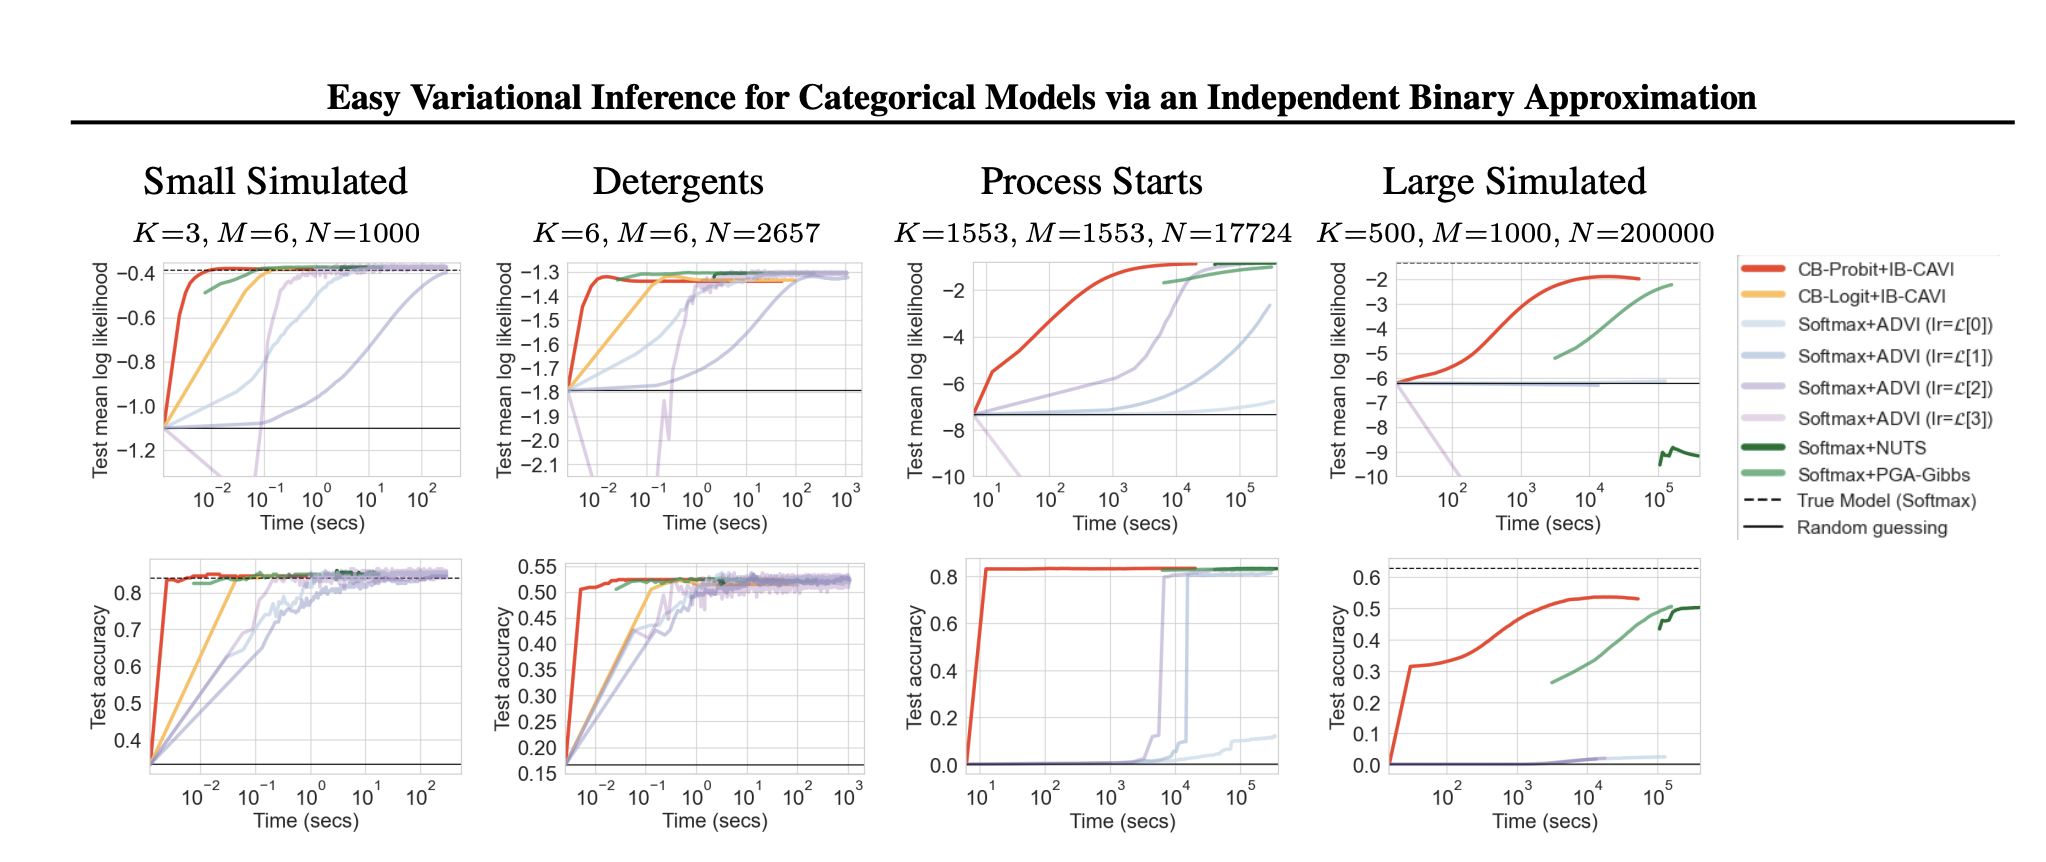
\includegraphics[width=.9\textwidth]{images/icml} 
%    \end{figure}
%   \citebottom{\hfill Wojnowicz et al. (2022). \textit{International Conference of Machine Learning (ICML)}. \hfill }
%	
%\end{frame}



%\begin{frame}{Discrete math: Example application}
%
%
%Find subtle DNA copy number alterations to support \textbf{early cancer detection}.
%
%\centering \includegraphics[width=.2\textwidth]{images/amplification_deletion} 
%
%\citebottom{Image from: Nabavi \& Zare (2022).}
%
%\end{frame}
%
%
%\begin{frame}
%\begin{columns}[T,onlytextwidth]
%    \begin{column}{0.4\textwidth}
%        \centering
%        \vspace{1in}
%        \Large How to detect changepoints within heavy noise?
%     \end{column}
%    \begin{column}{0.6\textwidth}	
%	 \begin{center}
%	  \includegraphics[width=0.5\linewidth]{images/sample_0} \\
%	\includegraphics[width=0.5\linewidth]{images/sample_1}
%	\end{center}
%    \end{column}
%\end{columns}
%
%\end{frame}
%
%
%\begin{frame}
%
%\large \centering
%The solution to this problem uses almost every content area we're covering in this course
%
%\vfill 
%\begin{itemize}
%	\item Discrete probability 
%	\item Counting
%	\item Complexity (Big-O notation)
%	\item Recursions
%	\item Graph theory
%	\item Proof techniques
%\end{itemize}
%\end{frame}



\agendaframe{6}

\begin{frame}
\begin{figure}

\includegraphics[width=0.7\textwidth]{images/tips_for_reading_math}
\end{figure}
%
\begin{figure}
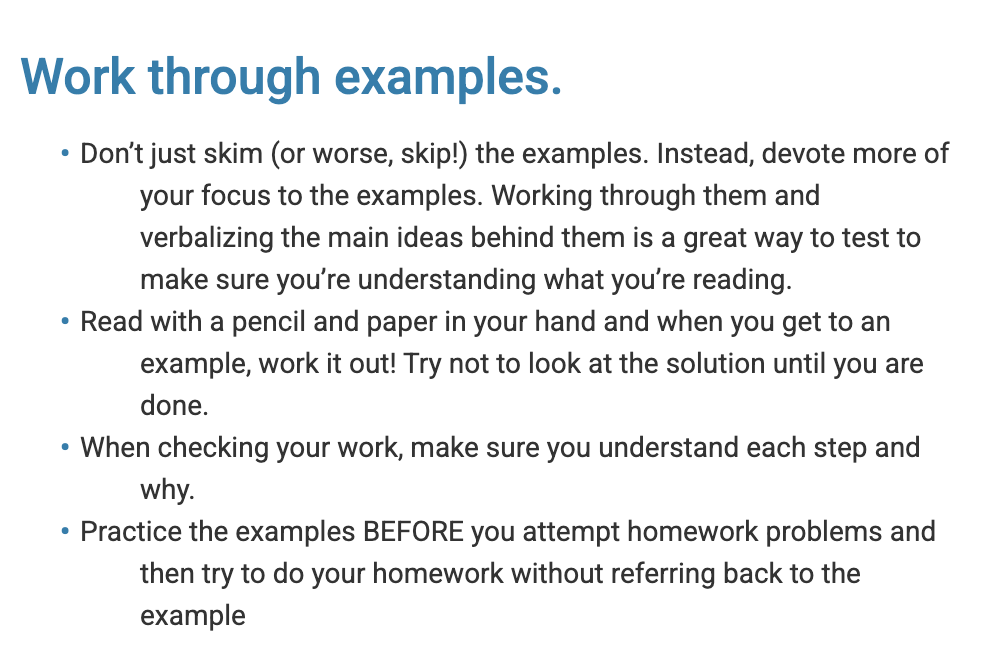
\includegraphics[width=0.7\textwidth]{images/work_through_examples}
\end{figure}
\bottomtext{\hfill Source: \url{https://learningcenter.unc.edu/tips-and-tools/readingmathtexts/}.}
\end{frame}







\end{document}